\documentclass[12pt,titlepage,french]{article}
\usepackage{babel}
\usepackage{graphicx}
\usepackage[margin=2.5cm]{geometry}

\usepackage[hidelinks]{hyperref}

\usepackage[utf8]{inputenc}
\usepackage[T1]{fontenc}
\pagestyle{plain}

\usepackage{booktabs,makecell,tabu}
\renewcommand\theadfont{\bfseries}

\linespread{1.5}

\begin{document}
%\renewcommand{\thesection}{\arabic{section}} % utilisé pour spécifier la numérotation des sections

\begin{titlepage}
\newcommand{\HRule}{\rule{\linewidth}{0.5mm}}
\center

  
\includegraphics[width=0.45\textwidth]{./image2.png}\\[1cm]
   
  
\includegraphics[width=0.45\textwidth]{./image1.png}


\HRule \\[0.4cm]
{ \huge \bfseries Cahier des charges \\[0.15cm] }
Classification colorimétrique de nuages de points 3D
\HRule \\[1.5cm]
Ronan Collier,
Mathieu Letrone,
Tri-Thien Truong
\\[1cm]
\today \\ [1cm]
Version 1.1
\end{titlepage}

\section{Introduction}

Nous tenons avant tout à remercier l'entreprise TagLabs, et plus particulièrement M. Yan KOCH, pour sa disponibilité et de sa confiance pour l'élaboration de ce projet.

Nous remercions également notre tuteur de stage, M. Nicolas NORMAND, pour son temps accordé sur ce projet.

\subsection*{Contexte general du projet dans l'entreprise}

Taglabs est une jeune entreprise créée il y a deux ans par Yan Koch. L’entreprise s’inscrit dans le domaine de la modélisation 3D d’ouvrages. Ils proposent la modélisation et l’exploitation de nuages de points. Mais, ils travaillent surtout en interne sur un logiciel « ScanSap », le but de ce logiciel est d’exploiter les nuages de points 3D avec efficacité et simplicité inégalées.

Voulant continuer leur développement dans ce domaine encore nouveau, l'entreprise cherche maintenant à améliorer leurs outils, afin de compléter l'exploitation des nuages de points. L'ensemble de ces fonctionnalités permettent à leurs clients de pouvoir analyser un environnement en numérique, à un instant précis (qui sera sous la forme d'un scan de nuages de points). Par exemple, une entreprise peut avoir le besoin d'avoir un scan d'une de leur usine, afin d'analyser le positionnement de leurs machines, les potentielles fuites au niveau des tuyaux, etc.

L'équipe qui sera à la charge de ce projet est composé de trois étudiants en informatique à Polytech Nantes. Dans le cadre de la quatrième année dans la formation d'ingénieur informatique, nous devons réaliser un projet transversal avec une entreprise.
\subsection*{MOA}

\noindent\begin{tabu} to \textwidth {X[c]X[c]X[c]X[c]}\toprule
   \thead{Qui}&\thead{Rôle}&        \thead{Mail}&\thead{Mobile}\\\toprule
      Yan Koch&   Président&  yankoch@taglabs.fr&    0660239733\\\midrule
Robin Kervadec&   Ingénieur&rkervadec@taglabs.fr&    0619656021\\\bottomrule
\end{tabu}

\subsection*{MOE}

\noindent\begin{tabu} to \textwidth {X[c2]X[c]X[c3]X[c]}\toprule
     \thead{Qui}&\thead{Rôle}&                       \thead{Mail}&\thead{Mobile}\\\toprule
Tri-thien Truong& Développeur&tri-thien.truong@etu.univ-nantes.fr&    0631193663\\\midrule
   Ronan Collier& Développeur&   ronan.collier@etu.univ-nantes.fr&    0666847162\\\midrule
 Mathieu Letrone& Développeur& mathieu.letrone@etu.univ-nantes.fr&    0789662916\\\bottomrule
\end{tabu}

\subsection*{Tuteur}

\noindent\begin{tabu} to \textwidth {X[c2]X[c2]X[c3]X[c]}\toprule
     \thead{Qui}&\thead{Rôle}&                       \thead{Mail}&\thead{Mobile}\\\toprule
Nicolas Normand& Département informatique&Nicolas.Normand@univ-nantes.fr&    0240683207\\\bottomrule
\end{tabu}

\section{Modèle du domaine / vocabulaire}

La solution devra permettre d’isoler, classifier un élément dans le nuage de points pour une meilleure visibilité et compréhension. Pour cela, la classification se basera selon la plage de couleur
\begin{itemize}
	\item  s'il est déjà en couleur: on applique le filtre de plage colorimétrique pour isoler les éléments (exemple: isoler les tubes proches du blanc).\par

	\item  s'il est en intensité de gris, on passe d'abord par de la fausse couleur, étape qui permet à l'utilisateur de mieux percevoir le nuage, puis on applique le filtre par plage colorimétrique.\par

\end{itemize}

Vocabulaire :

TODO

\section{Besoins fonctionnels}

\noindent\begin{tabu} to \textwidth {p{0.15\textwidth}X[c2]X[c2]X[c3]}\toprule
     \thead{MoSCoW}&\thead{Fonctions}&\thead{Critères}&\thead{Flexibilité}\\\toprule
M &Lire un fichier de données contenant un nuage de points
& Le nuage doit être visible à l'écran. La solution doit pouvoir lire un fichier au format ASCII
& Visibilité complète du nuage de points donné. L'extension du fichier ainsi que l'ordre des points et des données de ces points est laissé libre.\\\midrule
M & Modifier une couleur selon une intensité définie
& Affichage dans la lecture du scan
& La couleur qui sera affichée devra correspondre à la couleur voulue\\\midrule
C & Segmenter le nuage de points en ensembles plus petits
& Afficher une partie du nuage de points
& \\\midrule
M &Isoler un élément dans un nuage de points donné, selon sa plage de couleur 
& Les points isolés doivents appartenir à la plage de couleur désirée.
Les points appartenant à l'élément ciblé mais de teintes différentes doivents également extraits (ombrages, réflexion, ...).
& \\\midrule
M & Exporter le nuage de points
& Le nuage devra garder les modifications effectuées
& L'extension du fichier ainsi que l'ordre des points et des données de ces points est laissé libre.\\\bottomrule
\end{tabu}

\subsection*{Cas d'utilisation}

\begin{center}
    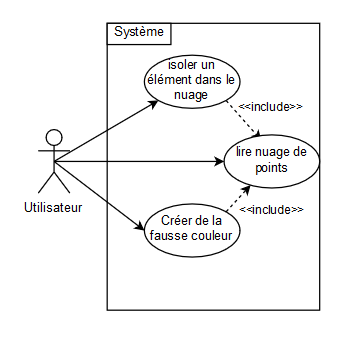
\includegraphics{usecase.PNG}
\end{center}

\subsection*{User story}

\begin{enumerate}
    \item Isoler un élément dans le nuage de points
    
En tant qu'utilisateur du logiciel, je veux isoler un élément dans le nuage de points afin d'afficher à l'écran uniquement l'élément voulu selon sa couleur.

\textbf{Tests d'acceptation :}

\begin{enumerate}
    \item Scénario 1
    
Etant donné que j'ai affiché un nuage de points via un fichier\\
Quand je clique sur l'option pour isoler un élément\\
Alors une interface avec un color picker apparaît\\
Quand je sélectionne une plage de couleur\\
Et que je clique sur le bouton Valider\\
Alors Le nuage de points n'affiche uniquement que les points respectant la plage d'intensité de couleur.


\end{enumerate}
\item Réaliser de la fausse couleur sur un nuage de points en intensité
En tant qu'utilisateur du logiciel, je souhaite faire resortir des variations de gris du nuage afin de mettre en lumière de nouveaux éléments et faciliter la compréhension.
\begin{enumerate}
    \item Scénario 1
    
Étant donné que j'ai affiché un nuage de point via un fichier\\
Quand je clique sur l'option fausse couleur\\
Alors une interface avec un outil utilisateur\\
Quand je l'utilise\\
Et que je clique sur valider\\
Alors le nuage de point s'affiche en fausse couleur.
\end{enumerate}
\end{enumerate}


\section{Besoins non fonctionnels}

\noindent\begin{tabu} to \textwidth {X[c]X[c3]}\toprule
     \thead{Fonctions}&\thead{Commentaires}\\\toprule
Traitement des problèmes de "mouchetage"
& Dans un premier temps, le mouchetage ne sera pas pris en compte dans le traitement du nuage de points.
\\\midrule
Sélection de la plage de couleurs à extraire 
& Le programme fournit une interface graphique comportant un "color-picker" permettant à l'utilisateur d'effectuer la sélection.\\\midrule
Performances de l'ordinateur
& A cause des nuages de points, il est nécessaire d'avoir des ordinateurs un minimum performants. Cela veut donc impliquer le fait que le programme développé nécessitera aussi un ordinateur performant.\\\midrule
Fichiers en entrée
& L'utilisation du programme devra vérifier la conformité des scans que l'on nous fournira.\\\midrule
Language utilisé
& Il n'y a aucun language requis par le client, nous utiliserons Python, un langage maitrisé par toute l'équipe de développement et adapté à la manipulation de données telles que des nuages de points\\\bottomrule
\end{tabu}

\section{Evolution potentielle des besoins}

Les besoins énoncés ici concernent des fonctionnalités que le client voudrait ajouter sur un de leur logiciel déjà existant (ScanSap). A termes, il voudra donc les ajouter directement sur ce dernier, au lieu d'avoir une utilisation externe comme prévu dans le cadre de notre projet transversal.

Il y a donc déjà des fonctionnalités existantes, sur des logiciels tels que Cloud Compare, permettant de nous aider sur nos besoins fonctionnels (par exemple, la lecture d'un scan, la segmentation etc.). La majeur partie à développer ici sera le changement de couleur et l'isolation de points.

Il sera peut-être possible que la réalisation des tâches sera plus rapide que prévu. Des nouveaux besoins pourront donc apparaître chez le client, afin d'améliorer les outils ou de développer des nouvelles fonctionnalités qui n'ont pas été abordé jusqu'ici.


\section{Limites du projet}

La correction des erreurs et artefacts des fichiers fournis en entrée du programme ne font pas partie du projet.
De même que la visualisation du nuage de points directement depuis le programme. Cette fonctionalité est assurée par le logiciel de l'entreprise, plus performant. Cette fonctionnalité peut être présente mais uniquement à des fins de test.

\section{Risques}

Incapacité à distinguer les éléments de façon efficace dû à des artefacts ou manques d'informations sur une zone du nuage de points.\\
Impact trop important du mouchetage sur la qualité de la segmentation.\\
Panne du matériel de travail.

\section{Plannings}
\subsubsection*{Planning général}
\begin{center}
    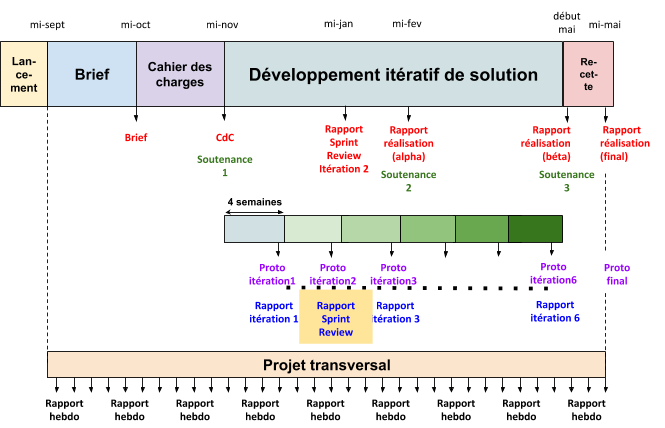
\includegraphics[width=\textwidth]{planning.png}
    \label{fig:Planning général}
\end{center}
L'ensemble du Projet transversale se déroule de septembre à mi-mai. Et il est jaloné par quatre grandes étapes : 
\begin{enumerate}
    \item De mi-septembre à mi-octobre : Réalisation du Brief
    \item De mi-octobre à mi-novembre : Réalisation du Cahier des charges 
    \item De mi-novembre à début mai : Développement itératif de la solution
    \item Mi-mai : Restitution du projet
\end{enumerate}

\subsubsection*{Planning détaillé}

\begin{center}
    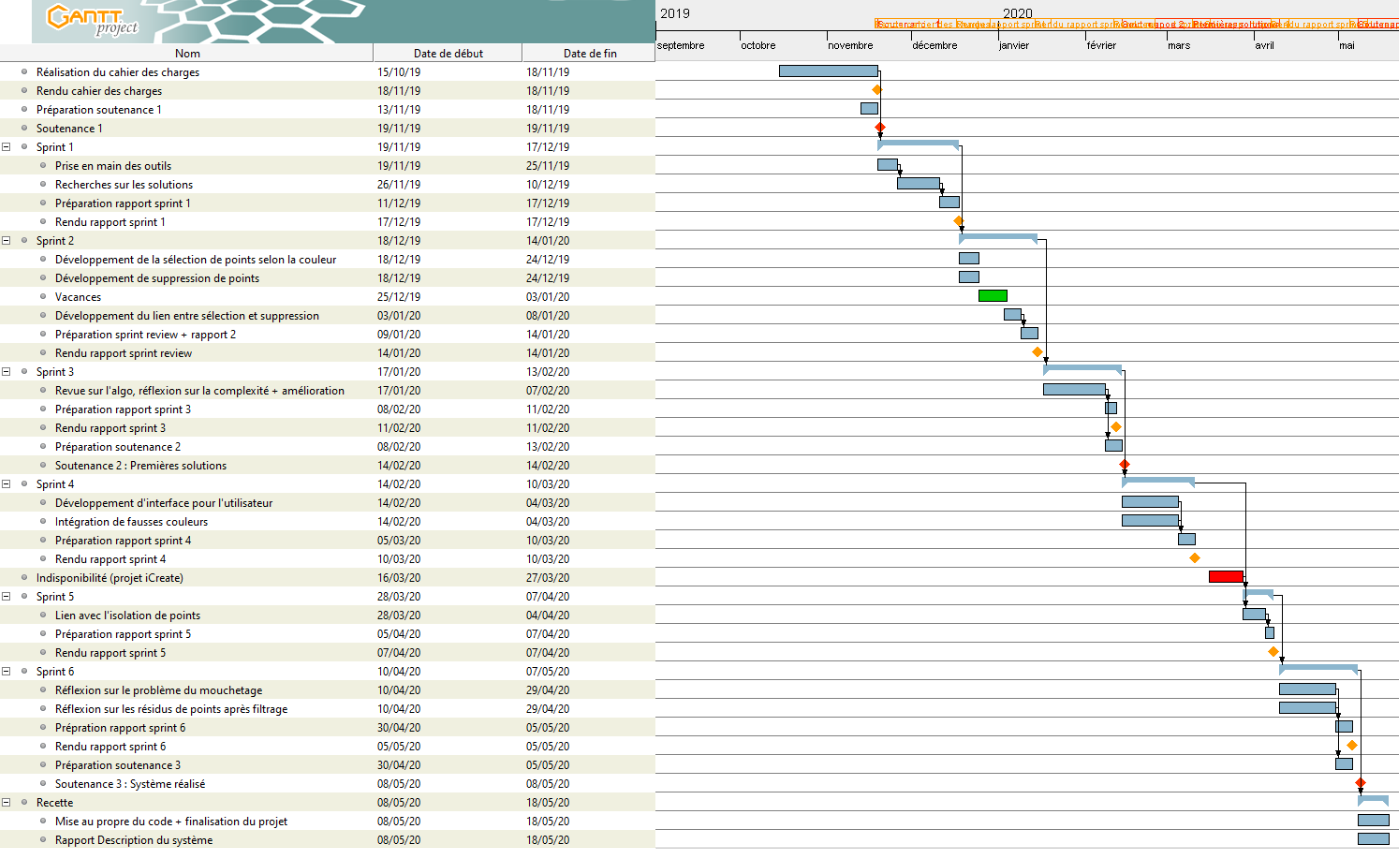
\includegraphics[scale=0.5,angle=90,origin=c]{gantt.png}
    \label{fig:Planning détaillé}
\end{center}


\section{Gestion de projet}

Pour la bonne réalisation du projet en mode agile, certaines responsabilités devront être respecté du côté de la MOE et de la MOA.

La MOE se tient de fournir au client un suivi continu du projet. En effet, via les différents sprints qui seront réalisés, le client aura une visibilité sur l'évolution de la réalisation du projet, via des rapports, des prototypes et démonstrations. Ces évolutions seront disponibles à la fin de chaque sprint.

Quant à la MOA, elle se tient de garder un contact avec la MOE, et de respecter les rendez-vous convenus. De plus, elle pourra fournir des exemples de nuages de points permettant de réaliser des tests sur le projet. Si des conseils ou autres informations permettant le bon développement du projet peuvent être communiqués, la MOE pourra alors prendre contact avec la MOA pour se tenir informé.

\section{Connaissances utiles}

TODO
\end{document}
